

\required{Detailed Proposal Information}
\section{Statement of Work (SOW)}
The project's aim is to develop a minaturized high-sensitivity, low-noise magnetic gradiometer. Our approach is to mimic the mechanism found in magnetosomes, the specialized cells four from bacteria to higher vertebrates such as fish and birds (see \ref{sec:inno}). This is comprised of four main tasks: modeling and simulation, microfabrication process design, circuit design, and device manufacture and testing. Each Phase (1,2,3) will include these four tasks.
\begin{table}[h!]
\centering
  \begin{tabular}{|c||c|c|c|}
    \hline
    Metric & Phase 1 & Phase 2 & Phase 3 \\
    \hline
    \hline
    Power consumption & 150 mW & 50 mW & 100 mW \\
    \hline
    Sensor Volume & 3x3x10 cm & 1x1x7 cm & 1x1x7 cm \\
    \hline
    Control Electronics Volume  & N/A & N/A & < 20cm$^2$ \\
    \hline
    Ambient Magnetic Field & $\pm$ 100 $\mu$T & $\pm$ 100 $\mu$T & $\pm$ 100 $\mu$T \\
    \hline
    Ambient Operating Temperature & N/A & 0$^{\circ}$ C to 50$^{\circ}$ C & 0$^{\circ}$ C to 50$^{\circ}$ C \\
    \hline
    Gradient Full-scale Range & 1 nT/cm & 1 nT/cm & 1 nT/cm \\
    \hline
    Gradient Sensitivity & 10 fT/cm/$\sqrt{Hz}$ & 3 fT/cm/$\sqrt{Hz}$  & 1 fT/cm/$\sqrt{Hz}$ \\
    \hline
    Gradient Accuracy & 100 fT/cm & 30 fT/cm & 10 fT/cm \\
    \hline
    Total Field Range & 100 $\mu$T & 100 $\mu$T & 100 $\mu$T \\
    \hline
    Total Field Sensitivity & 100 pT/$\sqrt{Hz}$ & 30 pT/$\sqrt{Hz}$  &  10 pT/$\sqrt{Hz}$ \\
    \hline
    Total Field Accuracy & 1 nT & 500 pT & 100 pT \\
    \hline
    Data Rate & 100/s & 200/s & 500/s \\
    \hline
    3 dB Bandwidth & 200 Hz & 400 Hz & 1000 Hz\\
    \hline
  \end{tabular}
\caption{Design objectives, by phase.}
\label{table:obj}
\end{table}

\subsection{Phase 1 Tasks}

AMBIIENT Phase 1 will demonstrate sensor functionality and performance in a laboratory
setting meeting the performance metrics as indicated in Table \ref{table:obj}. 

\subsubsection{Modeling and simulation}\label{sec:p1:em}
\begin{itemize}
\item The objective in this phase is to simulate the MEMS device, taking into account geometry, material properties, and multiphysics interactions, in order to determine the range of acceptable design options for a single element. Multiple options can be fabricated for real-world testing. 
\item Our approach here is to initially specify geometry and physical properties by hand calculation, then investigate more deeply in a finite-element multiphysics solver.
\item This task will be accomplished at UF by Joaquin Casanova.
\item Completion of this task is specified by successful simulation of the MEMS device that meets the physical requirements specified in the BAA.
\item Deliverables include successful simulation results and design parameters.
\item No government equipment is required.
\item To reduce risk of later failure due to non-manufacturability, this task will be accomplished within fabrication constraints specified by the MEMS team at UF. This ensures the design is physically realizable. In parallel, other sensing modalities could be explored in the case that the MEMS cantilever is not practical.
\end{itemize}
\subsubsection{Microfabrication}\label{sec:p1:mf}
\begin{itemize}
\item The objective in this phase is to develop a microfabrication strategy (materials, deposition, patterning) that can meet the requirements found from simulation.
\item Our approach here is to find a range of dimensional constraints and material types that could be physically realizable, and use those options to guide simulation and design of a sensor.
\item This task will be accomplished at UF by Dr. YK Yoon.
\item Completion of this task is successful specification of a microfabrication plan for the sensor described by the simulation results.
\item Deliverables include successful microfabrication plan.
\item No government equipment is required.
\item To reduce risk of later failure due to non-manufacturability, this task will be accomplished with parallel investigating of alternative MEMS sensing modalities.
\end{itemize}
\subsubsection{Circuit design}\label{sec:p1:cir}
\begin{itemize}
\item The objective in this phase is to develop a PCB-based detection circuit which amplifies and digitizes the the voltage produced by the MEMS elements. In addition to a COTS circuit, we will simultaneously begin investigation and design of an SiGe IC that can be used in later phases.
\item Our approach here is to drive the cantilevers at their resonant frequency to enhance sensitivity, amplifying the signal, then demodulate. Banks of sensors will be individually addressable. 
\item This task will be accomplished at TTU by Dr. Changzi Li.
\item Completion of this task is specified by successful design of a circuit capable of amplifying and digitizing MEMS output voltage with input-referred voltage noise low enough to meet the overall sensitivity requirement.
\item Deliverables include successful design and prototype of the circuit, usable with the fabricated MEMS sensor head, using COTS components.
\item No government equipment is required.
\item To reduce risk of later failure due to excessive noise, this task will investigate only specifically low-noise designs. Dynamic element matching will permit cancellation of manufacturing variation cancellation. The Phase 1 circuit will be completed with COTS components.
\end{itemize}
\subsubsection{Manufacture and testing}
\begin{itemize}
\item The objective in this phase is to construct the MEMS design using microfabrication processes and design developed in \ref{sec:p1:em},\ref{sec:p1:mf}, which includes pads for connection to circuitry.
\item Our approach here is to test the circuit and sensor independently and together after manufacturing as in \ref{sec:p1:mf}. Multiple MEMS design options can be fabricated for testing.
\item This task will be accomplished at UF by Dr. Yoon and Dr. Joaquin Casanova.
\item Completion of this task is specified by successful construction and testing of a sensor head, which satisfies Table \ref{table:obj}, using the circuitry developed in \ref{sec:p1:cir}.
\item Deliverables include successful prototype of the sensor and sensor electronics.
\item No government equipment is required.
\item To reduce risk of failure, fabrication will begin early in Phase 1, enabling us to revise our design to reduce manufacturing defects orenhance sensivity. 
\end{itemize}

\subsection{Phase 2 Tasks}
  
AMBIIENT Phase 2 will develop and demonstrate an integrated sensor head meeting the
performance and SWaP metrics of Table \ref{table:obj}, and including all vacuum, photonic, and thermal
control components.

\subsubsection{Modeling and simulation}\label{sec:p2:em}
\begin{itemize}
\item The objective in this phase is to optimize the MEMS device, to decrease size, increase sensitivity, and construct in arrays, based on results from the Phase 1. Phase 1 measured results will be compared to simlation to refine accuracy of simulations and account for effects that may not have been considered.
\item Our approach here is to first compared measured vs. simulated results, update our simulations, and then use the refined model to optimize a new design.
\item This task will be accomplished at UF by Joaquin Casanova.
\item Completion of this task is specified by successful simulation of the MEMS device that meets the physical requirements specified in the BAA for Phase 2.
\item Deliverables include successful simulation results and design parameters.
\item No government equipment is required.
\item To reduce risk of later failure due to non-manufacturability, this task will be accomplished within fabrication constraints specified by the MEMS team at UF, and considering the results of the Phase 1 testing. This ensures the design is physically realizable and modeling is accurate.
\end{itemize}
\subsubsection{Microfabrication}\label{sec:p2:mf}
\begin{itemize}
\item The objective in this phase is to optimize the microfabrication process, through material selection and process design, considering problems encountered in Phase 1.
\item Our approach here is to improve the material selection and process design over Phase 1, in conjunction with Phase 2 simulations. For instance, incorporating higher-energy magnetic materials, or denser interconnects.
\item This task will be accomplished at UF by YK Yoon.
\item Completion of this task is specified by successful fabrication of the Phase 2 MEMS design.
\item Deliverables include successful MEMS sensor, with pads for connection to the Phase 2 circuit.
\item No government equipment is required.
\item To reduce risk of later failure due to non-manufacturability (as a result of interconnect density, or damping effects, for instance), this task will also investigate an architecture with fewer, larger sensors.
\end{itemize}
\subsubsection{Circuit design}\label{sec:p2:cir}
\begin{itemize}
\item The objective in this phase is to optimize the PCB-based circuit based on the Phase 1 results and test this with a MEMS array, and incorporate the amplifier design into an integrated circuit, for testing with the Phase 2 MEMS array.
\item Our approach here is to take the Phase 1 circuit design, modifying based on the modified MEMS design, and design from this an integrated circuit, to reduce size. SiGe is a likely process choice due to low noise.
\item This task will be accomplished at TTU by Changzhi Li.
\item Completion of this task is specified by successful design and fabrication of a sensor amplification IC.
\item Deliverables include successful IC and design.
\item No government equipment is required.
\item To reduce risk of later failure due to missing deadlines, or circuit/MEMS mismatch, preliminary IC design will begin in Phase 1. Additionally, multiple designs can be incorporated into one IC.
\end{itemize}  
\subsubsection{Manufacture and testing}\label{sec:p2:test}
\begin{itemize}
\item The objective in this phase is to manufacture the IC and MEMS for Phase 2, and test these in the lab.
\item Our approach here is to do microfabrication at UF, and outsource the IC fabrication. The IC and MEMS sensor will be tested separately, and then together, once the functionality of each is established. The IC can be tested independently with dummy sources to verify function, and the MEMS sensor can be tested with a COTS circuit first. Varying field strength, frequency, and gradient using Helmholtz coils can establish sensitivity and noise floor of the sensor.
\item This task will be accomplished at UF by Dr. Yoon and Dr. Joaquin Casanova.
\item Completion of this task is specified by successful construction and testing of a sensor head, which satisfies Table \ref{table:obj}, using the circuitry developed in \ref{sec:p2:cir} and MEMS in \ref{sec:p2:em}.
\item Deliverables include successful prototype of the sensor and sensor electronics.
\item No government equipment is required.
\item To reduce risk of failure, fabrication will begin early in Phase 2, enabling us to revise our design to reduce manufacturing defects orenhance sensivity.
\end{itemize}

\subsection{Phase 3 Tasks}
AMBIIENT Phase 3 will demonstrate a fully integrated gradiometer comprising all control
electronics, power conditioning, and packaging, meeting all performance metrics of Table  \ref{table:obj}

\subsubsection{Modeling and simulation}\label{sec:p3:em}
\begin{itemize}
\item The objective in this phase is to optimize the MEMS device, to decrease size and increase sensitivity, based on results from the Phase 2. Phase 2 measured results will be compared to simulation to refine accuracy of simulations and account for effects that may not have been considered. The Phase 3 design will be completed with circuit integration specifically in mind.
\item Our approach here is to first compared measured vs. simulated results, update our simulations, and then use the refined model to optimize a new design.
\item This task will be accomplished at UF by Joaquin Casanova.
\item Completion of this task is specified by successful simulation of the MEMS device that meets the physical requirements specified in the BAA for Phase 3.
\item Deliverables include successful simulation results and design parameters.
\item No government equipment is required.
\item To reduce risk of later failure due to non-manufacturability, this task will be accomplished within fabrication constraints specified by the MEMS team at UF, and considering the results of the Phase 2 testing. This ensures the design is physically realizable and modeling is accurate.
\end{itemize}
\subsubsection{Microfabrication}\label{sec:p3:mf}
\begin{itemize}
\item The objective in this phase is to optimize the microfabrication process, through material selection and process design, considering problems encountered in Phase 2.
\item Our approach here is to improve the material selection and process design over Phase 2, in conjunction with Phase 2 simulations. For instance, incorporating higher-energy magnetic materials, or denser interconnects. Additionally, the Phase 3 MEMS and Phase 3 circuit will be integrated into the same substrate, and packaged. The Phase 3 IC will be sliced and bondined onto a common substrate with the MEMS.
\item This task will be accomplished at UF by YK Yoon and at TTU by Changzhi Li.
\item Completion of this task is specified by successful fabrication of the Phase 3 MEMS design.
\item Deliverables include successful MEMS sensor, with integrated Phase 3 sensor.
\item No government equipment is required.
\item To reduce risk of later failure because the IC and MEMS can't be integrated as part of the same substrate, we will also pursue the option of completing each separately and connecting. 
\end{itemize}
\subsubsection{Circuit design}\label{sec:p3:cir}
\begin{itemize}
\item The objective in this phase is to optimize the SiGe IC based on the Phase 2 results and refined Phase 3 design, and full-scale integration of the IC and MEMS sensor array.
\item Our approach here is to take the Phase 2 circuit design, modifying based on the modified MEMS design, adding an ADC,  and design from this a single integrated circuit, to reduce size. 
\item This task will be accomplished at TTU by Changzhi Li.
\item Completion of this task is specified by successful design and fabrication of a sensor amplification IC.
\item Deliverables include successful IC and design.
\item No government equipment is required.
\item To reduce risk of later failure due to missing deadlines, or circuit/MEMS mismatch, preliminary Phase 3 IC design will begin in Phase 2. Additionally, multiple designs can be incorporated into one IC.
\end{itemize}  
\subsubsection{Manufacture and testing}\label{sec:p3:test}
\begin{itemize}
\item The objective in this phase is to manufacture the IC and MEMS for Phase 3, and test these in the lab.
\item Our approach here is to do MEMS and the IC fabrication at UF, if possible. The IC and MEMS sensor will be tested separately, and then together, once the functionality of each is established. The IC can be tested independently with dummy sources to verify function, and the MEMS sensor can be tested with a COTS circuit first. Varying field strength, frequency, and gradient using Helmholtz coils can establish sensitivity and noise floor of the sensor.
\item This task will be accomplished at UF by Dr. Yoon and Dr. Joaquin Casanova.
\item Completion of this task is specified by successful construction and testing of a sensor head, which satisfies Table \ref{table:obj}, using the circuitry developed in \ref{sec:p3:cir} and MEMS in \ref{sec:p3:em}.
\item Deliverables include successful prototype of the sensor and sensor electronics.
\item No government equipment is required.
\item To reduce risk of failure, fabrication will begin early in Phase 3, enabling us to revise our design to reduce manufacturing defects orenhance sensitivity.
\end{itemize}

\section{Innovative Claims}\label{sec:inno}

Our approach is to design a sensor based on a magnetoreceptive mechanism used in nature - magnetite crystals torqued by external magnetic fields open ion channels in the cell wall. To mimic this, we propose a microfabricated MEMS sensor, with a layer of magnetic material on top of piezo electric cantilevers. When forced with an exernal field, torque induced on the magnet create stress in the piezo, and thus a voltage is produced. There are three advantages to this approach. First, microfabrication allows for a small size. Second, by orienting individual sensing elements in anti-series order, the output is natively a gradiometer. Third, by selecting the resonant frequency of the cantilever carefully, we can create a gradiometer which outputs a spectrogram directly. Though fluxgates can be microfabricated and function as gradiometers, they suffer a size/sensitivity tradeoff. Microfabricated atmonic magnetometers are sensitive but don't function natively as gradiometers. Other micro-scale magnetometers, namely Lorentz-type, which operate on a similar mechanism, are not yet sensitive enough and haven't been used as frequency-domain gradiometers, as in the proposed design.

\section{Detailed Technical Approach}

\subsection{Motivation and previous work}

Magnetometers serve an important role in investigating biologically generated electromagnetic fields, such as those created by neuronal currents, or geological magnetic fields. Typically, magnetometers are unable to achieve high sensitivity in an ambient, unshielded environment - getting to femtotesla level sensitivity requires magnetic shield and cryogenic sensors, such as SQUID \cite{lenz2006magnetic}. The novel spin relaxation free magnetometer has been minaturized and achieves less than 10 fT/$\sqrt{Hz}$, but still requires shielding and lacks directional sensitivity \cite{shah2013compact}. Fluxgates have achieved pT level resolution at small size, but this is insufficient for biomagnetic field measurement \cite{sasada2002orthogonal,uchiyama2014highly,sasada2014fundamental} 

Lorenz-type magnetometers (which translate magnetic fields into mechanical actuation of a magnet or current carrying wire) have been built in MEMS substrates, but are as yet insufficiently sensitive and require shielding \cite{sinha201627,kyynarainen20083d,kumar2015ultra,thompson2009parametrically}

Three of the proposers (Drs. Lin, Li, and Casanova) have been involved in previous DARPA work on the Mind Electromagnetic Localization Device (MELD) project, which involved designing, fabricating, and testing low-field magnetometers and the concomitant circuitry and software. Our experience in this field has given us useful experience and equipment, so we are familiar already with this pitfalls and challenges associated with the previously mentioned approaches. Dr. Yoon has direct experience in developing advance microfabrciation processes and applications (
\cite{yoon2003reduced,yoon2006multidirectional}), leading us to consider a different approach: mimicking the magnetometry found int nature on the cellular level.

\begin{wrapfigure}{L}{.65\textwidth}
\centering
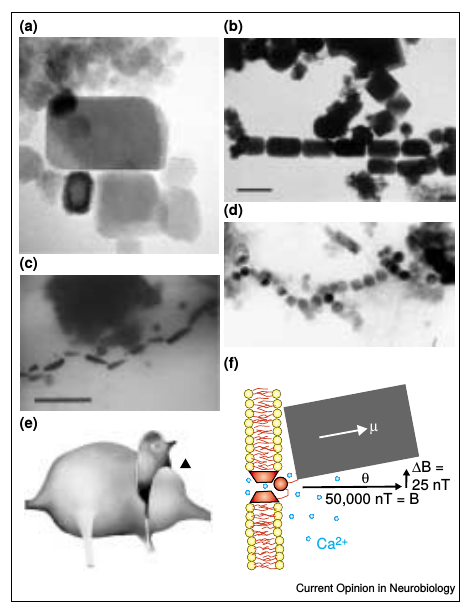
\includegraphics[width=0.5\textwidth]{kirsh2001}
\caption{Magnetosomal mechanism \cite{kirschvink2001magnetite}.}
\label{fig:magnetosome}
\end{wrapfigure}

In nature, many organisms have a sense of magnetoreception used for navigation, from magnetotactic bacteria to birds. Two mechanisms have been proposed: a spin-selective (and thus field-sensitive) chemical reaction rate, or magnetite crystals which are actuated by external fields and activate ion channels in the cell membrane (Figure \ref{fig:magnetosome})\cite{johnsen2005physics,dodson2013radical,kirschvink2001magnetite}. Measurements of these magnetosomes show a magnetic dipole moment of up to 100fA/m$^2$ \cite{hanzlik2002pulsed,eder2012magnetic}.


\subsection{Biomimetic sensor design}

\begin{figure}
\centering
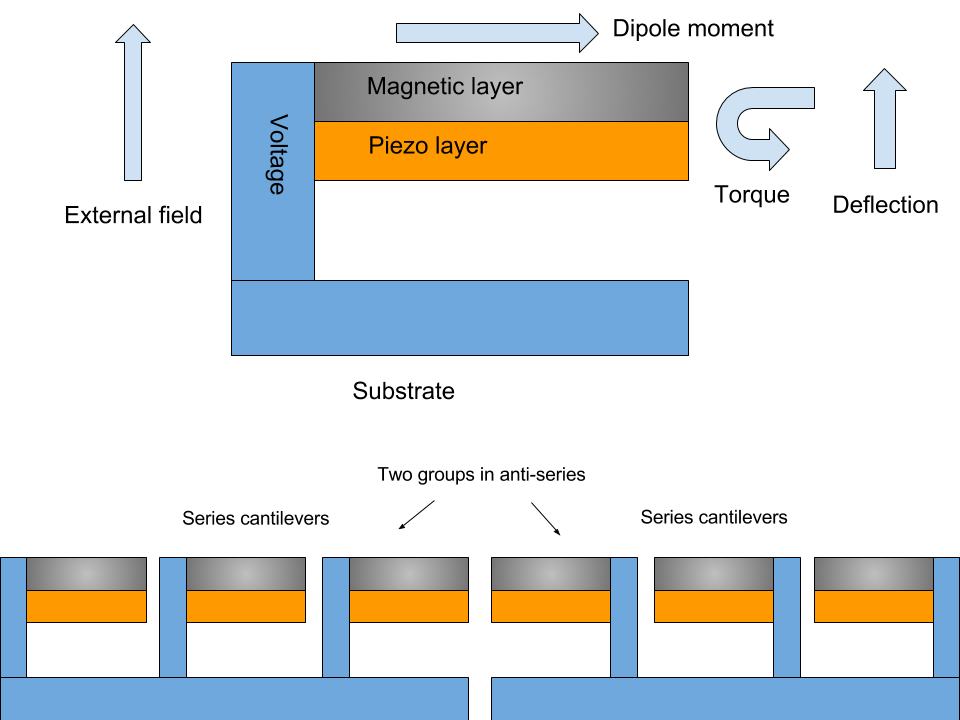
\includegraphics[width=0.7\textwidth]{biomag}
\caption{Diagram of proposed design.}
\label{fig:diagram}
\end{figure}

Our approach is to mimic the approach found in magnetosomes, with some key modifications so that is frequency-selective and functions inherently as a gradiometer and thus does not require shielding. The closest biomimetic sensor is a flow sensor which uses ferromagnetic cilia to detect microfluidic flow rates \cite{alfadhel2014magnetic}.

%\begin{wrapfigure}{L}{.65\textwidth}
%\centering
%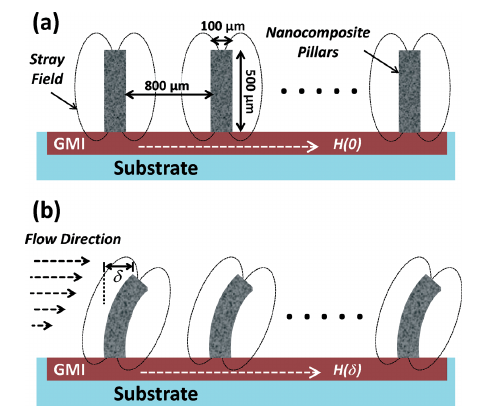
\includegraphics[width=0.5\textwidth]{cilia}
%\caption{Magnetic cilia flow sensor \cite{alfadhel2014magnetic}.}
%\label{fig:cilia}
%\end{wrapfigure}

To acomplish this, we propose layering a permanent magnetic layer on top of piezoelectric cantilevers. The torque induced on the magnetic layer generates stress in the piezo layer, and thus a voltage and charge. For an estimate of the sensitivity of this type of sensor, we perform a basic analysis. The moment $N$ induced on the magnetic layer with moment $\vec{\mu}$ and field $\vec{B}$ is:

$$  N=\vec{\mu} \times \vec{B} $$

Interpreted as a point load ($M/L$) at the cantilever tip, this moment causes a stress distribution on a cantilever of length L, thickness t, second moment I, piezoelectric voltage constant $g_{31}$, and modulus E, at point (x,y), of

$$ \sigma=\frac{Ny(L-x)}{LI} $$

and $n$ in series generates a voltage

$$ V=\frac{\int_0^L\int_{-t/2}^{t/2}\left|\frac{Ny(L-x)}{LI}g_{31}n\right|dydx}{L} $$

Two features are possible from the cantilever design: frequency selection and gradiometery. As in \cite{shen2008design}, a cantilever has a resonant frequency, which can be modified through geometrical parameters. Peak response will be achieved at this frequency. By selecting many cantilevers of different dimensions, each corresponding to a separate output, the magnetometer output is a spectrometer. Many cantilevers at the same resonance in series generate a larger voltage; in anti-series, the difference is taken, thus functioning as a gradiometer with very high spatial resolution (Figure \ref{fig:diagram}).

The noise floor of magnetic materials is governed by Barkhausen noise - the random flipping of magnetic domains \cite{butta2012sources}; this noise is characterized as a flux noise level. The flux noise can be converted into a magnetic moment noise, and thus moment noise. Piezo noise floor is largely a function of piezo losses \cite{levinzon2004fundamental}. Additionally, there is the input-referred noise of any amplifier. With conservative estimates for all of these, and two anti-series banks of 30 cantilevers each with dimensions 400x40x3 $\mu$m, the sensitivity level is less than 10 fT/cm/$\sqrt{Hz}$.

 Even though biological magnetoreception is limited to nT sensitivity, our design will allow us to surpass this. First, by careful selection of materials (such as Co-Pt or rare-earth magnets) \cite{coey2010magnetism, arnold2009permanent} we can have much higher magnetic dipole moment, and thus higher moment. Second, by careful selection of geometery, we can employ parametric resonance \cite{van2006resonant}. Third, by using many elemens in series and summing, we can increase signal-to-noise ratio (SNR). Finally, using two banks of cantilevers in series in anti-series, we both boost the voltage and create a high resolution gradiometer.

 Some potential pitfalls include effects of viscous damping (limiting mechanical vibration at resonance), demagnetization factor (due to the particular geometry of the magnetic layer), and layer separation from stress differentials (if strain at the interface betwwen layers is not equal, they can peel apart). To assess these more closely, multiple physical effects, with non-linear, anisotropic materials must be considered simultaneously, for a complex geometry. A large part of the MEMS sensor design process must therefore be completed in simulation, allowing us to determine the impact of the above effects. Additionally, we can optimize the geometry and material selection for maximum reponse. Key design variables include the coercivity and remanance of the magnetic layer, the piezoelectric coefficients of the piezoelectric layer, the Young's modulus of each, and the length, width, and thickness of the cantilever. The physics of the system can be described by the PDEs for magnetostatics, mechanical deformation, fluid flow, and the piezoelectric constitutive relations:

 $$ \nabla \vec{B} = 0$$

 $$ \vec{B} = \mu_o(\vec{H}+\vec{M}(\vec{H}))$$

where $\vec{B}$ is the magnetic flux,$\vec{H}$ the sum of external and internal fields, and $\vec{M}$ the magnetization.
 
 $$ EI\frac{\partial^4u}{\partial^4x}+m(x)\frac{\partial^2u}{\partial^2t}+\gamma\frac{\partial u}{\partial t}=q(x)$$

 $$ EI\frac{\partial^2N(x)}{\partial^2x} = -q(x)$$
 
$$ N(x) = \vec{\mu}(x) \times \vec{B_{ext}}, \vec{\mu}(x) = \vec{M}(x)dxdydz $$

$$\sigma_{xx}(x,y)  = N(x,y)y/I(x)$$

where $N$ is the moment, $q$ is load, $u$ is vertical displacement of the beam, $EI$ is the modulus/moment product, $m$ is mass per length, $\gamma$ is damping, and $\sigma$ is stress. This can (and should) be expanded to consider stress in multiple axes.
Finally, to relate field $\vec{E}$, strain $\vec{S}$, displacement field $\vec{D}$, and stress $\vec{\sigma}$, in the piezo layer:
 $$S_{ij} = s_{ijkl}\sigma_{kl}+d_{kij}E{k}$$

$$D_i=d_{ikl}\sigma_{kl}+\epsilon_{ik}E_{k}$$
 
Together, these relations allow us to estimate resonance, stress, and sensitivity of our sensor. FeniCS provides an open-source finite-element multiphsics solver \cite{dupont2003fenics}; though less user-friendly, it is flexible, and free, and sufficient for our needs.


\subsection{Microfabrication process}

Microfabrication processes are capable of constructing the above-described sensor. This consists of two main fabrication tasks: piezo cantilever construction, and magnetic material integration. PZT has a high voltage coefficient and is highly suitable for the piezo elements \cite{tadigadapa2009piezoelectric} and can be deposited with pulsed laser deposition or solution-based deposition and patterned with chemical etching or ion etching. Rare-earth magnetic materials, such as alloys of Sm-Co, offer high magnetic energy product at room temperature and can be integrated into MEMS using sputtering or pulsed laser deposition \cite{arnold2009permanent}. However, patterning of these materials is slow, using wet etching or ion-beam milling. A likely strategy will be to use a sacrificial polymer pattern, depositing electrodes, piezo, then magnet layers, and then etching the sacrificial layers. 

The process described in \cite{shen2008design} can be used for our task, with an additional step to apply the magnetic layer. To construct an energy-harvesting piezo cantilever, \cite{shen2008design} used a four-mask process.


\begin{figure}
\centering
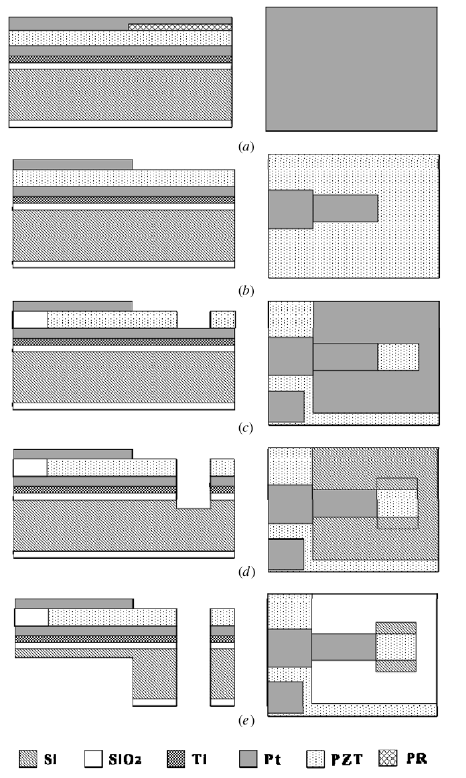
\includegraphics[width=0.75\textwidth]{cantifab}
\caption{Cantilever fabrication \cite{shen2008design}.}
\label{fig:fab}
\end{figure}

\begin{itemize}
\item SiO2 was grown on both sides of a silicon wafer.
\item Ti and bottom electrode Pt were deposited by sputtering, followed by sol-gel deposition of PZT (Fig. \ref{fig:fab}(a)).
\item A top Pt electrode was patterned by a first mask and deposited by a lift-off process (Fig. \ref{fig:fab}(b)):
  \begin{itemize}
  \item A sacrificial photoresist layer was deposited and patterned
  \item Pt was deposited on the patterned photoresist
  \item The sacrificial layer was removed
  \end{itemize}
\item The bottom electrode (the first Pt layer) was exposed from the topside with a second mask and etched with inductively coupled plasma reactive ion etching (RIE) (Fig. \ref{fig:fab}(c)).
\item The cantilever was patterned from above with a third mask via RIE (Fig. \ref{fig:fab}(d)).
\item The cantilever proof mass (used here to enhance resonance) was patterned and released through backside RIE (Fig. \ref{fig:fab}(e)
\end{itemize}

In our case, we would need an additional ferromagnetic layer on top. This could be deposited, then patterned and etched, or deposited according to some pattern, followed by annealing. In either case, of critical importance is selected a material whose magnetic properties are optimal (high remanence and coercivity), whose annealing temperatures are compatible with the other materials, and which can be etched easily enough. It should also maintain magnetic properties within the operating temperature range (has a high Curie temperature), and be oxidation resistant (for instance, some rare-earth magnets are prone to oxidation and must be tungsten-coated).

\subsection{Circuit design}
 
\begin{figure}
\centering
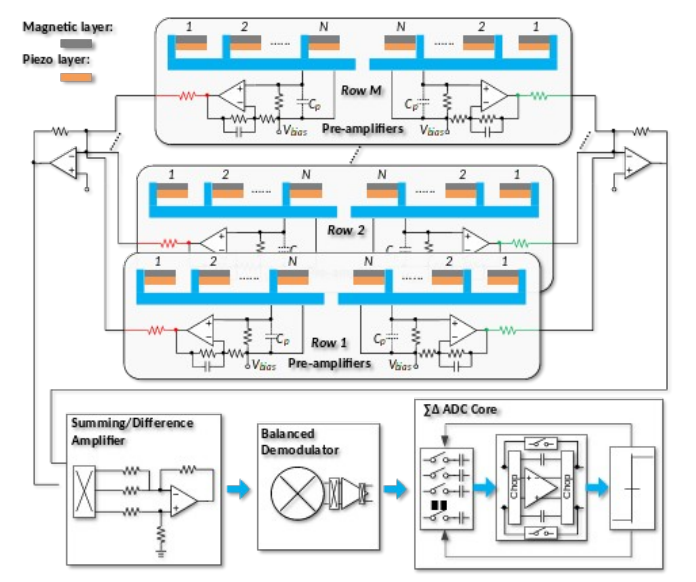
\includegraphics[width=0.65\textwidth]{system}
\caption{System design.}
\label{fig:system}
\end{figure}

From circuits and systems point of view, this could be modeled using a very-large-scale oversampling sensing architecture. A simple example is laid out as follows: 

Assuming a sensor of area $A$ generates a signal of $S$, and it has intrinsic noise of $N_i$. In comparison, two sensors each with an area of $A/2$ would each generate a signal of $S/2$ and noise of $N_i/2$. When the two $A/2$ sensors are combined, their total signal will be $S$. But since the noises from the two $A/2$ sensors are uncorrelated, the combined total noise will be:

$$\sqrt{(N_i/2)^2+(N_i/2)^2} = N_i/\sqrt(2) $$

Therefore, splitting a sensor into two with equal sizes will result in a factor of $\sqrt{2}$ increase in the signal-to-noise ratio (SNR). Likewise, splitting a sensor into an array of $M$ small units that sum up to the same total size would lead to a factor of $\sqrt{2}$ increase to the SNR. Because of this “oversampling gain” to the SNR, magnetosomes with thousands of magnetite crystals are able to have a superb sensitivity to small fluctuations of magnetic field, which can hardly be achieved by conventional man-made tools. 

Ideally, if a sensor can be split into an infinite number of miniaturized elements, it would approach the capability of magnetosomes to achieve ultra-high field sensitivity. On the other hand, it is the most desirable to implement this bio-inspired oversampling mechanism in the analog front-end because any added back-end circuitry would introduce parasitics and noise that would otherwise hinder the effectiveness of the ideal oversampling theory. Inspired by this bio-mechanism of oversampling, we propose to combine the magnetic/piezo cantilevers in groups, and use low-noise amplifiers to pick up signals directly from the elements. The low-noise amplifiers will be reconfigurable in summing and difference modes to detect total field and field gradient. An overview of the system is shown in \ref{fig:system}.

Voltage-mode and charge-mode amplifications are two main approaches to signal conditioning of piezoelectric sensors. Voltage-mode amplification is useful when the amplifier is very close to the sensor and thus minimal parasitic capacitance is presented by the interconnection between the sensing device and the amplifier input. Charge-mode amplification is useful when the amplifier is remote to the sensor because it is robust against parasitic capacitance of interconnections. Depending on the characterization and optimization of the MEMS device front-end, the team is ready to investigate both approaches and fully integrate the final solution with special circuit techniques for the optimal performance. 

\subsubsection{Voltage-mode approach}

The simplified structure for voltage-mode amplifiers is depicted in Fig. 1, represented by the circuits that directly interface with each row of the MEMS device. Depending on the fabricated and optimized MEMS size, either one or multiple amplifiers in parallel will be implemented for each row to collect the piezoelectric voltage signal. The goal of using multiple amplifiers in parallel is to enhance the SNR because of the benefit of oversampling. However, constraint exists due to the area available under the MEMS device. The circuit team will work closely with the device team in this project to determine the ideal placement of local voltage-mode amplifiers in Phase I of this project, and compare the performance with the charge-mode approach discussed next.  

\subsubsection{Charge-mode approach}

\begin{wrapfigure}{R}{0.5\textwidth}
\centering
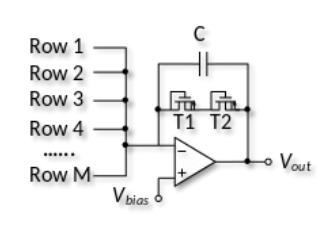
\includegraphics[width=0.4\textwidth]{cmos}
\caption{Charge-mode amplifier with pseudo-resistor feedback and summing capability.}
\label{fig:cmos}
\end{wrapfigure}

Charge-mode amplifier approach will also be investigated because it has advantages in handling interconnect parasitics and the convenience of adding signals from different rows of the MEMS device together. Inspired by existing works in neural recording \cite{harrison2003low}, the team will use MOS-bipolar pseudo-resistors as the feedback resistors in the charge-mode amplifier. As shown in Fig. \ref{fig:cmos}, two back-to-back connected PMOS transistors (T1 and T2) that can easily achieve resistance of GOhm will be implemented as the feedback resistor of the charge-mode amplifier, enabling processing brain signals with a frequency as low as 0.025 Hz. With negative VGS, T1 and T2 function as diode-connected PMOS transistors. With positive VGS, the parasitic source–well–drain p-n-p bipolar junction transistor (BJT) is activated, such that T1 and T2 act as diode-connected BJTs. For small voltages across the pseudo-resistors, the small-signal resistance is extremely high and thus moves the corner frequency to low enough for bio-signal processing. On the other hand, a large voltage across the pseudo-resistors will reduce the small-signal resistance and result in a fast settling time for the amplifier. As a result, this pseudo-resistor-based design can amplify low-frequency signals down to the millihertz range while properly rejecting large DC offsets. The theoretical noise–power tradeoff limit, i.e., the noise efficiency factor, have already been derived and demonstrated by selectively operating MOS transistors in either weak or strong inversion \cite{harrison2003low}. The only potential drawback of this configuration is that the amplifier cannot have a large output swing, because otherwise the pseudo-resistors may become two diodes. However, this is not a concern for this work as the amplifier is implemented as pre-amplifier in the front-end, where signal to be handled is very weak.

\subsubsection{Re-configurable summing and difference amplifiers}

After the piezoelectric signal is captured by arrays of preamplifiers located near the MEMS devices, the obtained voltage signals will be further processed by a re-configurable summing and difference amplifier. This amplifier will be digitally controlled in real-time to either add or subtract signals coming from different regions of the fabricated device. This will enable both common-mode detection, which senses the total field, and differential-mode detection, which senses the field gradient.

One potential challenge for the summing and difference amplifier is the tradeoff between high sensitivity and large dynamic range. Being able to perform both summing and difference detection, as well as the existence of strong earth field, requires the amplifier to have a very large dynamic range. However, the DARPA specification also mandate high sensitivity for brain signal recovery. To this end, a 3-op-amp topology will be customized and implemented in GlobalFoundries 180-nm SiGe BiCMOS 7WL process for both low-noise and high-linearity operation. Bipolar PNP transistors will be utilized as the input buffer to minimize the input-referred noise. A programmable resistor array will be implemented between the outputs of the two first-stage amplifiers to provide a large tunable gain range. In a previous DARPA project (MELD – Mind Electromagnetic Localization Device), the team has evaluated various topologies and different semiconductor processes (e.g., SOI versus BiCMOS) for the amplifier of brain magnetic field detector, and verified through both Cadence simulation and fabricated chip measurement that the 3-op-amp topology with bipolar transistor input buffer offers the best combined sensitivity and linearity performance.

\subsubsection{Solution to low-frequency noise and device mismatch in electronics}

Because the magnetic field induced by brain activities not only is extremely weak, but also has very low frequencies (below 100 Hz), 1/f noise and device mismatch have significant impact to the success of the proposed work. To resolve the challenge, the bio-inspired MEMS device will operate at a resonant frequency which “carries” the signal of interest. A double-balanced demodulator featuring low noise at the baseband output, high rejection to harmonic distortion, and low LO/RF leakage will be implemented after the summing/difference amplifier to recover the field information of interest. 

After the signal is demodulated to the baseband, circuit techniques including dynamic offset cancellation, dynamic element matching (DEM), and chopping will be applied extensively to the remaining signal processing circuits to cancel the mismatch errors and low-frequency noises. On the data acquisition side, the analog-to-digital converter (ADC) is an important component for correctly interpreting the field information. Nyquist ADC accuracy is limited by the matching of components in ADCs, while oversampling ADCs, such as sigma-delta ADC, trade speed for resolution. Because brain signals have low frequencies, sigma-delta ADC is a very good candidate for precision sensing. Another advantage of sigma-delta ADC is that chopping technology and dynamic element matching are suitable for its architecture to minimize the impact of low-frequency noise and offset errors.


\section{Risk Analysis and Mitigation Plan}

\begin{table}[h!]
\centering
\begin{tabularx}{.85\textwidth}{|X||c|c|X|}
    \hline
    Risk & Probability & Impact & Plan\\
    \hline
    \hline
    Insufficient sensitivity in simulation & 3 & 10 & Optimize design architecture. \\
    \hline
    Best available MEMS processes infeasible & 4 & 10 & Begin design process within constraints of available processes. \\
    \hline
    Interconnects infeasible & 3 & 5 & Operate fewer, larger cantilevers \\
    \hline
    Viscous damping hurts sensitivity & 3 & 5 & Operate in vacuum packaging \\
    \hline
    Resonance frequency infeasibly high & 3  & 5 & Operate fewer, larger cantilevers \\
    \hline
    Fabrication unreliable/mismatch & 3 & 5 & Begin fabrication early, so process can be adjusted; dynamic element matching. \\
    \hline
    Sensitive to mechanical vibration & 3 & 5 & Use additional, non-magnetic cantilevers to cancel mechanical vibrations. \\
    \hline
\end{tabularx}
\caption{Risk matrix}
\label{table:risk}
\end{table}

There are several risks and challenges associated with this design. Most can be addressed simply by doing careful analysis of the problem within the range of constraints on materials and processes. Others (the density of interconnects, or resonant frequency, is too high) can be address by reducing the number of elements and increasing their size. Damping due to the viscosity of air could hurt sensitivity could be addressed by vacuum packaging the sensor head. Manufacturing mismatch of the sensing elements can be effectively removed by dynamic element matching, where the transducers are switched electronically to average out fabrication differences.

\section{Schedule and Milestones}

\begin{table}[h!]
\centering
  \begin{tabular}{|c||c|c|}
    \hline
    Phase & Milestone & Date\\
    \hline
    \hline
    1 & Cantilever simulation and design & \\
    \hline
    1 & Fabrication plan & \\
    \hline
    1 & Circuit design & \\
    \hline
    1 & Scale model design and testing & \\
    \hline
    \hline
    2 & Cantilever simulation and design & \\
    \hline
    2 & Fabrication plan & \\
    \hline
    2 & Circuit design & \\
    \hline
    2 & Microfabrication and testing & \\
    \hline
    \hline
    3 & Cantilever simulation and design & \\
    \hline
    3 & Fabrication plan & \\
    \hline
    3 & Circuit design & \\
    \hline
    3 & Microfabrication and testing & \\
    \hline
  \end{tabular}
\caption{Milestones schedule}
\label{table:sched}
\end{table}

Include a high-level Gantt chart outlining major technical tasks and measureable milestones
by phase. At a minimum, the schedule should include each SOW task of Volume 1, Section
II.A. Where risk reduction tasks are proposed, the schedule should include a milestone for
assessment and removal of redundant tasks.

\section{Test Plan}

To test, in Phase 1, the sensor will first be connected to the circuitry and powered to established basic functionality.  Prior to testing, noise from the Helmholtz coils, power supplies, and any other necessary signal generation sources will be characterized. Further, the sensor will be placed in a pair of Helmholtz coils driven with precision current sources, inside magnetic shield, so we can gauge accuracy and sensitivity in a controlled environment. Field gradient, intensity, and frequency will be swept over the range specified in \ref{table:obj}. Finally, the same test will be repeated in an unshielded environment. In each case, we will monitor power consumption, signal output, and mesure sensor and sensor control electronics volume. Subsequent phases will follow a similar testing protocol, except using specifications for those phases. Additionally, in Phases 2 and 3, where an IC will be developed and integrated with the sensor head, the IC will be tested independently to verify basic input/output functionality before slicing and bonding to the MEMS substrate.

\section{Results and Technology Transfer}

Our research team has demonstrated successful technology transfer to the government and private sectors in our work on wireless power, vital signs radar, and low-field magnetometry. UF's Office of Technology Licensing is very helpful in patenting and licensing new engineering developments from research.

The proposed work is highly amenable to technology transfer. The sensor and circuit design is novel and likely patentable, even if it fails to meet all requirements in the BAA. This can be considered fundamental research and thus not ITAR-controlled. Further, there is no private industry involvement, to any technology transfer is just between UF and DARPA.

\section{Ongoing Research}
Presently, Drs. Lin, Li, and Casanova are presently involved (until 6/2017) in a DARPA project for detection and inversion of MEG/EEG signals. They have worked on all phases, from sensor design to circuit design to inversion algorithm. Additionally, Drs. Lin and Li have worked exensively on vital signs radar, and Dr. Casanova has worked on electromagnetic sensors for agriculture and analytical chemistry. Dr. Yoon has conducted research in MEMS systems of all types, including piezoelectronics and magnetics. 

\section{Facilities}

Facilities at UF for sensor development and testing include magnetic shielding, circuit testing instrumentation (power supplies, oscillopes, function generators, VNA). For fabrication, the Nanoscale Research Facility at UF includes equipment for a variety of processes: plasma, vapor, and sputtering deposition, annealing, wafer bonding, wire bonding, UV and e-beam lithography, reverse ion etching, and wet etching.

PI Li’s research group at the Texas Tech University is located in a fully ESD-protected Microwave and Analog Circuits Laboratory. The PI has obtained full support from the Texas Tech University Provost Office and Electrical and Computer Engineering Department to establish this well-equipped lab and enhance the department’s research strength on the microwave, millimeter-wave, and analog circuits. Equipment includes high-frequency network analyzers, signal generators, spectrum analyzer, and oscilloscopes; software useful to this project includes Cadence, Altium, MATLAB, and Labview.

\section{Teaming/Proposer Accomplishments}

\begin{description}
\item[UF] The UF team incluldes the following personnel:
  \begin{description}
  \item[Jenshan Lin] will be project lead, and supervise work on the AMBIIENT project. His time commitment is 0\%. He received the B.S. degree in Electrophysics from National Chiao Tung University (NCTU), Hsinchu, Taiwan, R.O.C., in 1987, and the M.S. and Ph.D. degrees in Electrical Engineering from the University of California at Los Angeles (UCLA), in 1991 and 1994, respectively. His current research interests include sensors and biomedical applications of microwave and millimeter-wave technologies, wireless energy transfer and conversion, RF system-on-chip integration, and integrated antennas. Dr. Lin has authored or co-authored over 250 technical publications in refereed journals and conference proceedings. He holds 15 patents and has several other patent applications. Since joining University of Florida, he has graduated 22 PhD students. 
  \item[Joaquin Casanova] will conduct electromagnetic simulation and design of the MEMS sensor, and work with Dr. Yoon on process/material selection, and Dr. Li on requirements for the interface and control circuits. His commitment is 50\%. He received a B.S. and M.E. in Agricultural and Biological engineering in 2006 and 2007 from UF, and PhD in Electrical Engineering in 2010 from UF. His work has primarily focused on sensors and electromagnetic design, including wireless power, microwave remote sensing, agricultural sensors, analytical chemistry equipment design, and low-field magnetic sensing. He is currently a Research Assistant Professor in UF's Department of Electrical and Computer Engineering. 
  \item[YK Yoon] will guide selection of a microfabrication process and fabrication of the sensor. His commitment is 10\%. He received his BS and MS degrees in electrical engineering from Seoul National University in Korea. He also earned an MSEE degree from the New Jersey Institute of Technology, Newark, NJ in 1999 and the Ph.D. degree in electrical and computer engineering from the Georgia Institute of Technology, Atlanta, GA in 2004. He is currently an Associate Professor in the Department of Electrical and Computer Engineering at the University of Florida, Gainesville, FL. His current research interests include three dimensional (3-D) micromachining and nano fabrication; design and implementation of metamaterial for radio frequency (RF) and microwave applications; micromachined millimeter wave and terahertz antennas and waveguides; bio/microfluidic systems for the lab-on-a-chip applications; wireless telemetry systems for biomedical applications; and ferroelectric material development for high density memory devices and/or tunable RF devices.
  \end{description} 
\item[TTU] The TTU team includes:
  \begin{description}
  \item[Changzhi Li] will design the electronics for amplifying and digitizing the signals from the sensor head, working with Dr. Casanova to determine ciruit requirements. His time commitment is 10\%. He received the B.S. degree in electrical engineering from Zhejiang University, China, in 2004 and the Ph.D. degree in electrical engineering from the University of Florida, Gainesville, FL, in 2009.In the summers of 2007 and 2008, he worked at Alereon Inc., Austin, TX, on ultrawideband (UWB) transceiver. In the summer of 2009, he worked at Coherent Logix Inc., Austin, TX, on software-defined radio. His research interests include analog circuits, microwave circuits, and biomedical applications of microwave/RF.
  \end{description}
\end{description}
\required{Additional Information}

\bibliography{./casanova_ieee}
